\documentclass[10pt]{beamer}

\beamertemplatenavigationsymbolsempty

\usepackage{multicol}
\usepackage[czech, english]{babel}
\usepackage[utf8]{inputenc}
\usepackage[T1]{fontenc}
\usepackage{booktabs}
\usepackage[scale=2]{ccicons}

\usepackage{diagbox}
\newcommand{\labelkm}{\scriptsize \diagbox[width=24pt,height=15pt]
        {\raisebox{-0pt}{k}}{ m } }


\usepackage{tikz}

\usepackage{gnuplottex}

\usepackage{booktabs,longtable}%
\usepackage{colortbl}%
\newcommand{\evenrowcolor}{\rowcolor[gray]{0.925}}

\title{
Practical Exhaustive Generation of Small
Multiway Cuts in Sparse Graphs
}
\subtitle{}
\date{}
\author{Petr Hliněný and Ondřej Slámečka}
\institute{Faculty of Informatics, Masaryk University, Brno}

\begin{document}

\maketitle

\begin{frame}
	\frametitle{Accidents, disasters and roads}

	Going from A to B when suddenly\ldots
\end{frame}

\begin{frame}
	\frametitle{Accidents, disasters and roads}
	\noindent\makebox[\textwidth]{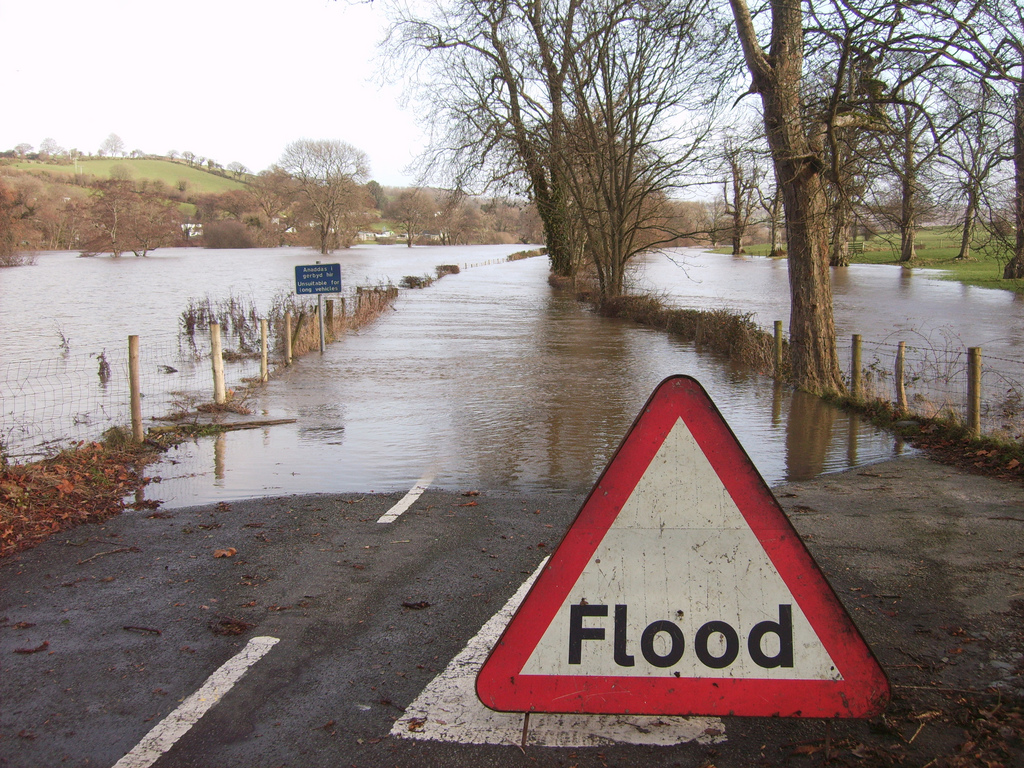
\includegraphics[width=\paperwidth]{images/flood.jpg}}
\end{frame}

\begin{frame}
	\frametitle{Accidents, disasters and roads}
	\noindent\makebox[\textwidth]{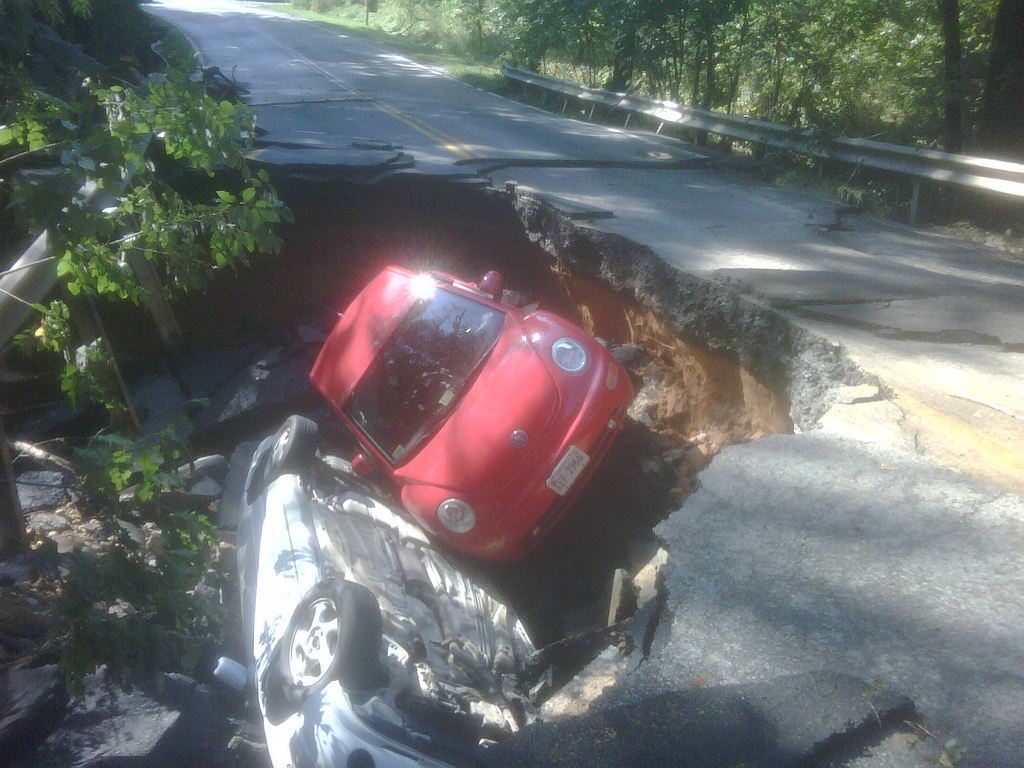
\includegraphics[width=\paperwidth]{images/road_wash.jpg}}
\end{frame}

\begin{frame}
	\frametitle{Accidents, disasters and roads}
	\noindent\makebox[\textwidth]{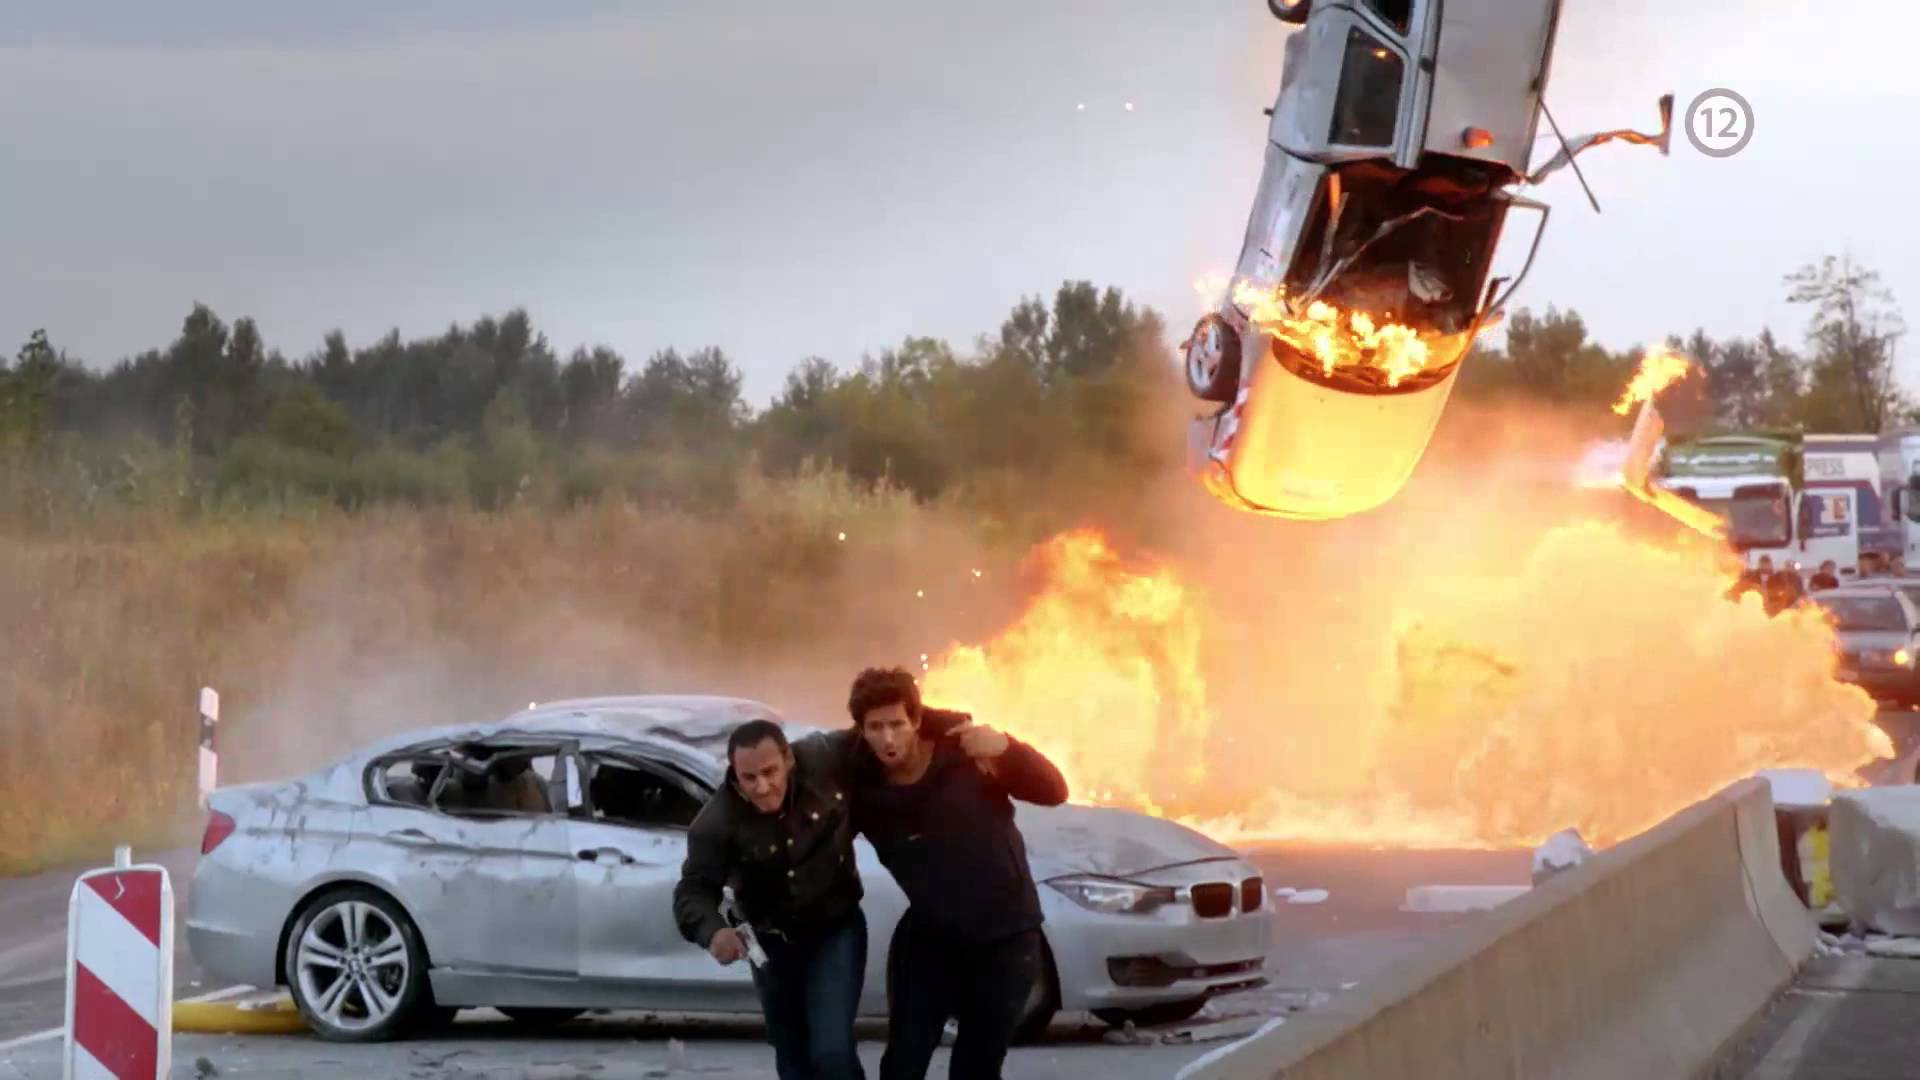
\includegraphics[width=\paperwidth]{images/kobra_11.jpg}}
\end{frame}

\begin{frame}
	\frametitle{Accidents, disasters and roads}

	Our way to B is cut.

	\bigskip

	Can this happen in situations other than travelling?
\end{frame}

\begin{frame}
	\frametitle{Networks}
	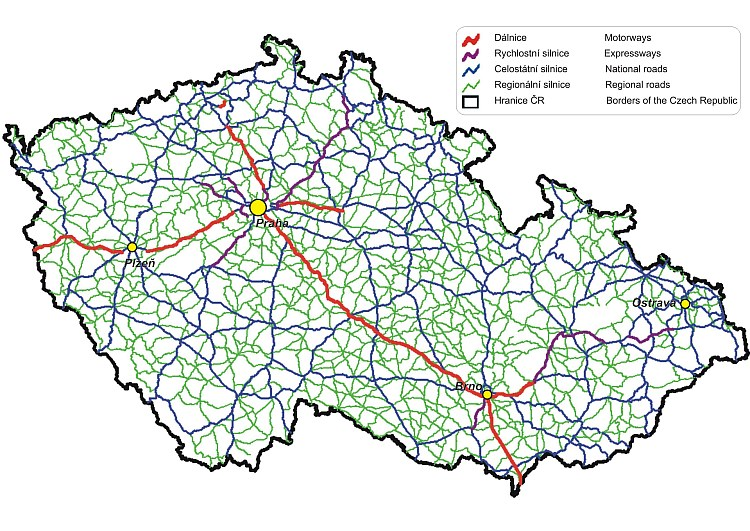
\includegraphics[width=\textwidth]{images/road_network.jpg}

	Not just roads. Also internet, electrical grid, bridges of Königsberg,\ldots
\end{frame}


\begin{frame}[fragile]
	\frametitle{The problem}


	For a given (sparse) graph $G = (V, E)$ find all the minimal (wrt.
	inclusion) sets $X \subseteq E$ such that, $G \setminus X$ has $k$
	connected components. \\

	\bigskip

	\bigskip
	\textbf{The problem is \#P-complete}

	We'll introduce parameter $m$ and limit our problem to finding all cuts $X$, such that $\lvert
	X \rvert \leq m$.

	\medskip

    For practical purposes there is no need for $m$ to be big.


\end{frame}

\begin{frame}[fragile]
	\frametitle{State of the art}

	\begin{itemize}
		\item The trivial approach: for each combination of up to $m$ edges count
    	the components of the graph without these edges.

		\item Reinelt, Wenger: Generating partitions
    	of a graph into a fixed number of minimum weight cuts. ``The cactus approach''
	\end{itemize}

    \bigskip

    When searching for previous work we had to filter out a lot papers
    dealing with seemingly similar but different problems.

    \medskip

	Our problem is not
	\begin{itemize}
		\item a single $s{-}t$ cut,
		\item minimal cuts with respect to set size,
		\item minimal cuts with respect to edge weight sum,
		\item with some specific condition (like planarity).
	\end{itemize}

\end{frame}

\begin{frame}[fragile]
    \frametitle{General idea}

	Let $M = (E, \mathcal{B})$ be a matroid. \\

	\bigskip

	If $C$ is a~circuit and $X$ is a cocircuit in a matroid $M$, then ${\lvert C \cap X \rvert \neq 1}$.

	\bigskip

	The algorithm:\\
    For all $b$ from an arbitrary basis of $M$ invoke \textsc{GenCocircuits}($\{b\}$).

	\textbf{\textsc{Function GenCocircuits}($X$)}
	\begin{enumerate}
		\item If $\lvert X \rvert > m$ \textbf{or} $E \setminus X$ contains no hyperplane of $M$, then halt here.
		\item Find a circuit $C$, such that $\lvert C \cap X \rvert = 1$.
		\item If there is no such $C$, then $X$ is a cocircuit.
		\item If there is such $C$, then for each $c \in (C \setminus X)$: \\
			\hspace{12pt} \textsc{GenCocircuits}($X \cup \{c\}$).
	\end{enumerate}

\end{frame}

\begin{frame}[fragile]
	\frametitle{Graph algorithm when $k$ equals $2$}

	Let $G = (V, E)$ be a graph. \\

	\bigskip

	If $X \subseteq E(G)$ is minimal cut and $C \subseteq E(G)$ a cycle,
    then $\lvert C \cap X \rvert \neq 1$.

    \bigskip

	The algorithm:\\
    For all $b$ from arbitrary spanning tree of $G$ invoke \textsc{GenCocircuits}($\{b\}$).

	\textbf{\textsc{Function GenCocircuits}($X$)}
	\begin{enumerate}
		\item If $\lvert X \rvert > m$ \textbf{or} vertices of any
            ``side'' of $X$ cannot be connected by a subgraph of $G$,
            then halt here.
		\item Find a cycle $C$, such that $\lvert C \cap X \rvert = 1$.
		\item If there is no such $C$, then $X$ is a minimal cut.
		\item If there is such $C$, then for each $c \in (C \setminus X)$: \\
			\hspace{12pt} \textsc{GenCocircuits}($X \cup \{c\}$).
	\end{enumerate}

\end{frame}



\begin{frame}
	\frametitle{Example}

    Colour one side of the future cut red and the other blue.
	\center
	\begin{multicols}{2}

        Input graph (spanning tree thick) \\
	\medskip
\begin{tikzpicture}[
  vertex/.style={draw,circle,minimum size=0.8cm},
  every node/.style={vertex},
  spanning_tree/.style={draw=black, ultra thick}
  ]
	\node (1) at (1,5) {1};
	\node (2) at (1,3) {2};
	\node (3) at (1,1) {3};

	\node (4) at (3,5) {4};
	\node (5) at (3,3) {5};
	\node (6) at (3,1) {6};

	\draw[spanning_tree] (1) -- (2);
	\draw[spanning_tree] (2) -- (3);

	\draw (4) -- (5);
	\draw (5) -- (6);

	\draw[spanning_tree] (1) -- (4);
	\draw[spanning_tree] (2) -- (5);
	\draw[spanning_tree] (3) -- (6);
\end{tikzpicture}
\\
$   $ \\

1. step \\
	\medskip
\begin{tikzpicture}[
  vertex/.style={draw,circle,minimum size=0.8cm},
  every node/.style={vertex},
  red_vertex/.style={draw=red},
  blue_vertex/.style={draw=blue},
  inx/.style={draw=black, ultra thick},
  onc/.style={draw=blue, thick}
  ]
	\node (1) at (1,5) {1};
	\node[blue_vertex] (2) at (1,3) {2};
	\node[red_vertex] (3) at (1,1) {3};

	\node (4) at (3,5) {4};
	\node[blue_vertex] (5) at (3,3) {5};
	\node[blue_vertex] (6) at (3,1) {6};

	\draw (1) -- (2);
	\draw[inx] (2) -- (3);

	\draw (4) -- (5);
	\draw[onc,<-] (5) -- (6);

	\draw (1) -- (4);
	\draw[onc, <-] (2) -- (5);
	\draw[onc, ->] (3) -- (6);
\end{tikzpicture}
 \\
 $X = \{ (2,3) \}$
	\end{multicols}

\end{frame}


\begin{frame}
	\frametitle{Example}

    Colour one side of the future cut red and the other blue.

	\center
	\begin{multicols}{2}

1. step \\
	\medskip
\begin{tikzpicture}[
  vertex/.style={draw,circle,minimum size=0.8cm},
  every node/.style={vertex},
  red_vertex/.style={draw=red},
  blue_vertex/.style={draw=blue},
  inx/.style={draw=black, ultra thick},
  red_edge/.style={draw=red, ultra thick},
  onc/.style={draw=blue, thick}
  ]
	\node (1) at (1,5) {1};
	\node[blue_vertex] (2) at (1,3) {2};
	\node[red_vertex] (3) at (1,1) {3};

	\node (4) at (3,5) {4};
	\node[blue_vertex] (5) at (3,3) {5};
	\node[blue_vertex] (6) at (3,1) {6};

	\draw (1) -- (2);
	\draw[inx] (2) -- (3);

	\draw (4) -- (5);
	\draw[onc, <-] (5) -- (6);

	\draw (1) -- (4);
	\draw[onc, <-] (2) -- (5);
	\draw[onc,->] (3) -- (6);
\end{tikzpicture}
 \\
 $X = \{ (2,3) \}$

1. step, 1. recursive call \\
	\medskip
\begin{tikzpicture}[
  vertex/.style={draw,circle,minimum size=0.8cm},
  every node/.style={vertex},
  red_vertex/.style={draw=red},
  blue_vertex/.style={draw=blue},
  inx/.style={draw=black, ultra thick},
  red_edge/.style={draw=red, ultra thick},
  onc/.style={draw=blue, thick}
  ]
	\node (1) at (1,5) {1};
	\node[blue_vertex] (2) at (1,3) {2};
	\node[red_vertex] (3) at (1,1) {3};

	\node (4) at (3,5) {4};

	\node[blue_vertex] (5) at (3,3) {5};
	\node[blue_vertex] (6) at (3,1) {6};

	\draw (1) -- (2);
	\draw[inx] (2) -- (3);

	\draw (4) -- (5);
	\draw[onc,<-] (5) -- (6);

	\draw (1) -- (4);
	\draw[onc, <-] (2) -- (5);
	\draw[inx] (3) -- (6);
\end{tikzpicture}
 \\
 $X = \{ (2,3), (3,6) \}$
	\end{multicols}

\end{frame}

\begin{frame}
	\frametitle{Example}

    Colour one side of the future cut red and the other blue.
	\center
	\begin{multicols}{2}

		1. step (back from recursive call) \\
	\medskip
\begin{tikzpicture}[
  vertex/.style={draw,circle,minimum size=0.8cm},
  every node/.style={vertex},
  red_vertex/.style={draw=red},
  blue_vertex/.style={draw=blue},
  inx/.style={draw=black, ultra thick},
  red_edge/.style={draw=red, ultra thick},
  onc/.style={draw=blue, thick}
  ]
	\node (1) at (1,5) {1};
	\node[blue_vertex] (2) at (1,3) {2};
	\node[red_vertex] (3) at (1,1) {3};

	\node (4) at (3,5) {4};
	\node[blue_vertex] (5) at (3,3) {5};
	\node[blue_vertex] (6) at (3,1) {6};

	\draw (1) -- (2);
	\draw[inx] (2) -- (3);

	\draw (4) -- (5);
	\draw[onc, <-] (5) -- (6);

	\draw (1) -- (4);
	\draw[onc, <-] (2) -- (5);
	\draw[onc] (3) -- (6);
\end{tikzpicture}
 \\
 $X = \{ (2,3) \}$

1. step, 2. recursive call \\
	\medskip
\begin{tikzpicture}[
  vertex/.style={draw,circle,minimum size=0.8cm},
  every node/.style={vertex},
  red_vertex/.style={draw=red},
  blue_vertex/.style={draw=blue},
  inx/.style={draw=black, ultra thick},
  red_edge/.style={draw=red, ultra thick},
  onc/.style={draw=blue, thick}
  ]
	\node (1) at (1,5) {1};
	\node[blue_vertex] (2) at (1,3) {2};
	\node[red_vertex] (3) at (1,1) {3};

	\node (4) at (3,5) {4};
	\node[blue_vertex] (5) at (3,3) {5};
	\node[red_vertex] (6) at (3,1) {6};

	\draw (1) -- (2);
	\draw[inx] (2) -- (3);

	\draw (4) -- (5);
	\draw[inx] (5) -- (6);

	\draw (1) -- (4);
	\draw[onc, <-] (2) -- (5);
	\draw[red_edge] (3) -- (6);
\end{tikzpicture}
 \\
 $X = \{ (2,3), (6,5) \}$
	\end{multicols}

\end{frame}


\begin{frame}
	\frametitle{Example}

    We would continue to finish the blue cycle and repeat the algorithm
    with another edge of the selected spanning tree.

    \bigskip

    The total result: a set of 2-way minimal cuts -- 2-bonds.
\end{frame}

\begin{frame}
	\frametitle{$k$-way cuts}

    Let $X$ be a 2-bond of a graph $G$. We can apply the algorithm
    recursively to each component of $G \setminus X$ to get all the
    3-bonds extending $X$.

    \bigskip

    The same matroid algorithm, only the matroid definition changes.
    In effect we have to choose a spanning forest.

\end{frame}

\begin{frame}
	\frametitle{$k$-way cuts example}

	\center
	\begin{multicols}{2}

	Input graph (SF thick) \\
	\medskip
\begin{tikzpicture}[
  vertex/.style={draw,circle,minimum size=0.8cm},
  every node/.style={vertex},
  spanning_tree/.style={draw=black, ultra thick}
  ]
	\node (1) at (1,5) {1};
	\node (2) at (1,3) {2};
	\node (3) at (1,1) {3};

	\node (4) at (3,5) {4};
	\node (5) at (3,3) {5};
	\node (6) at (3,1) {6};

	\draw[spanning_tree] (1) -- (2);

	\draw (4) -- (5);

	\draw[spanning_tree] (1) -- (4);
	\draw[spanning_tree] (2) -- (5);
	\draw[spanning_tree] (3) -- (6);
\end{tikzpicture}
\\
$  $ \\

1. step \\
	\medskip
\begin{tikzpicture}[
  vertex/.style={draw,circle,minimum size=0.8cm},
  every node/.style={vertex},
  red_vertex/.style={draw=red},
  blue_vertex/.style={draw=blue},
  inx/.style={draw=black, ultra thick},
  onc/.style={draw=blue, thick}
  ]
	\node (1) at (1,5) {1};
	\node (2) at (1,3) {2};
	\node[red_vertex] (3) at (1,1) {3};

	\node (4) at (3,5) {4};
	\node (5) at (3,3) {5};
	\node[blue_vertex] (6) at (3,1) {6};

	\draw (1) -- (2);

	\draw (4) -- (5);

	\draw (1) -- (4);
	\draw (2) -- (5);
	\draw[inx] (3) -- (6);
\end{tikzpicture}
\\
$X = \{(3,6)\}$ \\

	\end{multicols}

\end{frame}


\begin{frame}
	\frametitle{Permutations}

	Aren't some cuts produced in more than one permutation?

\begin{table}[H]
        \caption{The multiplicity of (repeatedly) generated bonds in the
        non-canonical generation algorithm.
         Zlín (top) and Olomouc (bottom)}
        \label{tab:repeated-canonical}
    \centering
        \begin{tabular}{c|rrrrrrrr}

    \hline

    \labelkm  &        3 &         4 &         5 &         6 &        7 \\[2pt]
    \hline
           3  &    3.112 &     4.309 &     6.092 &     8.152 &   10.465 \\
    \evenrowcolor
           4  &          &     9.706 &    13.642 &         - &        - \\

        \end{tabular}
{\vskip 3mm}
        \begin{tabular}{c|rrrrrrrr}

    \hline

     \labelkm &        3 &         4 &         5 &         6 &      7 \\[2pt]
    \hline
           3  &    2.840 &     4.038 &     5.536 &     7.491 &   9.739 \\
    \evenrowcolor
           4  &          &     8.817 &    12.432 &         - &      -  \\

        \end{tabular}
\end{table}


\end{frame}

\begin{frame}
	\frametitle{Canonical generation}

	The canonical construction path scheme. The idea of Brendan McKay used in {\tt nauty} (tool for generating groups of graph automorphisms).

	\bigskip

	The canonical form of a bond is chosen in advance. In each step of computation the algorithm evaluates whether the set $X$ can be extended, with the edge which is currently being processed, without breaking the canonical form.

\end{frame}

\begin{frame}
	\frametitle{A glitch in canonical generation}

	\begin{table}[H]
        \caption{
		The percentage of repeatedly generated bonds in the
		canonical generation algorithm.
	         Zlín (top) and Olomouc (bottom) Region
		%Zlín Region (left) and Olomouc Region (right)
		%Percentage of repeatedly generated bonds in the
		%canonical generation algorithm (top) and in the
		%non-canonical generation algorithm (bottom).
		%Zlín Region (left) and Olomouc Region (right)
		}
        \label{tab:repeated-canonical-failed}

        \begin{tabular}{c|rrrrrrrr}

    \hline

 \labelkm     &        3 &         4 &         5 &         6 &         7 \\[2pt]
    \hline
           3  &  0.972\% &   0.814\% &   1.618\% &   2.664\% &   3.715\% \\
    \evenrowcolor
           4  &          &   2.177\% &   1.950\% &   3.462\% &       -   \\


\iffalse
	\hline
	\noalign{\vskip 2mm}
	\hline
		   3  &  311.2\% &   430.9\% &   609.2\% &   815.2\% &   1046.5\% \\
    \evenrowcolor
           4  &          &   970.6\% &  1364.2\% &         - &        - \\
\fi

        \end{tabular}
{\vskip 3mm}
        \begin{tabular}{c|rrrrrrrr}

    \hline
 \labelkm       &         3 &         4 &         5 &         6 &         7 \\[2pt]
    \hline
             3  &   0.156\% &   0.253\% &   0.649\% &   1.049\% &   1.568\% \\
    \evenrowcolor
             4  &           &   0.352\% &   0.541\% &         -  &       -  \\
\iffalse
	\hline
	\noalign{\vskip 2mm}
	\hline
           3  &  284.0\% &   403.8\% &     553.6\% &     749.1\% &	973.9\% \\
    \evenrowcolor
           4  &          &   881.7\% &    1243.2\% &         - &      -  \\
\fi

        \end{tabular}

\end{table}


	\bigskip

	Not significant for practical purposes.

\end{frame}

\begin{frame}
	\frametitle{Practical implementation}

	Practical problems involved in the algorithm's running time.

	\begin{itemize}
		\item Choice of \textit{minimal spanning forest}.
		\item Choice of a certain variation of shortest path (minimizing triplets).
		\item Fast hyperplane existence testing (in graph terms: existence of two graphs interconnecting each side of a cut).
	\end{itemize}

	\bigskip
	Available online at \href{https://github.com/OndrejSlamecka/mincuts}{\url{https://github.com/OndrejSlamecka/mincuts}}.

\end{frame}

\begin{frame}
	\frametitle{Evaluation}

    \begin{table}[H]
        \caption{Running time of an implementation of the canonical
            generation in seconds. Zlín Region}
        \label{tab:runtimeZ}
        \centering
        \begin{tabular}{c|rrrrrrrr}

    \hline%\toprule
\labelkm&        2 &         3 &       4 &      5 &      6 &       7 &      8  \\[2pt]
	\hline%\midrule
     2  &      0.0 &       0.1 &       1 &      2 &      9 &     42  &  210     \\
    \evenrowcolor
     3  &      0.6 &      2.8  &     13  &     53 &   223  &    986  &  4604    \\
     4  &          &     29.5  &    198  &   1018 &   4771 &   21269 &  -       \\
    \evenrowcolor
     5  &          &           &   1156  &   9885 &  56847 &    -    & -        \\
        \end{tabular}
    \end{table}



    \begin{table}[H]
        \caption{Running time of an implementation of the canonical
            generation in seconds. Olomouc Region}
        \label{tab:runtimeO}
        \centering
        \begin{tabular}{c|rrrrrrrr}
    \hline%\toprule
\labelkm    &       2 &        3 &      4 &      5 &      6 &      7 &      8 \\[2pt]
    \hline
          2 &    0.1 &      0.3 &      1 &      5 &     16 &     69 &    305 \\
    \evenrowcolor
          3 &     3.0 &     10.4 &     61 &    235 &    921 &   3482 &  13342 \\
          4 &         &    158.3 &    781 &   6008 &     -  &      - &      - \\
    \evenrowcolor
          5 &         &          &   6205 &  43242 &     -  &      - &      - \\

        \end{tabular}
    \end{table}

\end{frame}

\begin{frame}
	\frametitle{Evaluation -- speedup with canonical generation}
 \begin{table}[H]
        \caption{Ratio of running times without
             and with canonical generation.
            Zlín (top) and Olomouc (bottom) Region}
        \label{tab:ratiocan-time}
        \centering
        \begin{tabular}{c|rrrrrrrr}

    \hline
\labelkm     &         2 &         3 &         4 &         5 &         6 &         7 \\
    \hline
          2  &     1.00  &      2.00 &      2.45 &      3.60 &       4.3 &      1.34 \\
    \evenrowcolor
          3  &      3.28 &      3.51 &      6.05 &      8.83 &     12.11 &     14.90 \\
          4  &           &      8.40 &     11.32 &     15.73 &         - &         - \\

\noalign{\vskip 3mm}
\hline
\labelkm &         2 &         3 &         4 &         5 &         6 &     7  \\
    \hline
      2  &      1.14 &      1.93 &      1.91 &      2.18 &      4.30 &  5.06  \\
      \evenrowcolor
      3  &      1.97 &      3.47 &      4.49 &      6.69 &      8.31 &  9.41  \\
      4  &           &      5.96 &     10.16 &     15.53 &         - &     -  \\

        \end{tabular}

	\end{table}


\end{frame}

\begin{frame}
	\frametitle{Evaluation}

\begin{table}[t]
	\centering
	\caption{The distribution of lengths of the path $P$ from the algorithm.
	Results of the computation on Zlín Region, $k = 3, m = 6$;
	on the left showing the second level of recursion of {\tt GenStage}, on the right
	the fifth level (the algorithm occasionally uses even longer paths in later {\tt
		GenStage} calls).}
	\label{tab:pathlengths}

	\begin{minipage}[b]{0.49\linewidth}\centering
		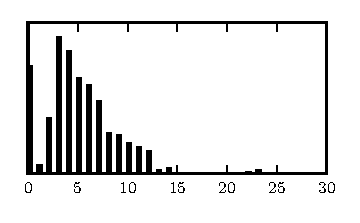
\includegraphics[scale=0.95]{fig/zlin_6_3_stage1_xsize2.pdf}
	\end{minipage}
	\begin{minipage}[b]{0.49\linewidth}\centering
		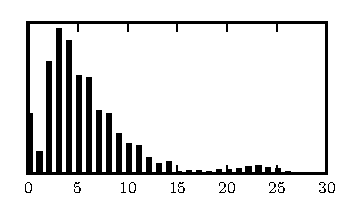
\includegraphics[scale=0.95]{fig/zlin_6_3_stage1_xsize5.pdf}
	\end{minipage}
\end{table}


\end{frame}

\begin{frame}
	\frametitle{Conclusion}

	Matroid setting provides an easy way to prove the correctness of the algorithm.
	Graph implementations exploit the structure of sparse graphs.

	\medskip

	The current speed is suitable for most practical needs of Transport Research Centre (Centrum Dopravního Výzkumu).

	\bigskip

	There is a lot of room for future work.
	\begin{itemize}
		\item How to approach canonical generation such that it is truly canonical?
		\item Compare our implementation with ``the cactus approach''.
		\item How to improve the implementation of the two current bottlenecks
			(hyperplane existence check and shortest path computation)?
	\end{itemize}

\end{frame}


\end{document}
